% !Mode:: "TeX:UTF-8"
%\documentclass[13pt]{beamer}
\documentclass[13pt, punct]{ctexbeamer}
%\usepackage[utf8]{inputenc}
%\parskip=8pt
%\lineskip=5pt

\titlegraphic{\includegraphics[width=2cm]{tjnu.jpg}}

\linespread{1.3}\selectfont
\makeatletter
\renewcommand\normalsize{%
	\@setfontsize\normalsize\@xpt\@xiipt
	\abovedisplayskip 1\p@ \@plus1\p@ \@minus6\p@
	\abovedisplayshortskip \z@ \@plus3\p@
	\belowdisplayshortskip 3\p@ \@plus3\p@ \@minus3\p@
	\belowdisplayskip \abovedisplayskip
	\let\@listi\@listI}
\makeatother


\usepackage{color}

%\usepackage{ctex}
%%%=== theme ===%%%
% \usetheme{Warsaw}
%\usetheme{Copenhagen}
%\usetheme{Singapore}
\usetheme{Madrid}
%\usefonttheme{professionalfonts}
%\usefonttheme{serif}
% \usefonttheme{structureitalicserif}
%%\useinnertheme{rounded}
%%\useinnertheme{inmargin}
\useinnertheme{circles}
%\useoutertheme{miniframes}
\setbeamertemplate{navigation symbols}{}
\setbeamertemplate{footline}[page number]


%\usepackage[style=numeric-comp, backend=bibtex, isbn=false, doi=false, url=false, eprint=false]{biblatex}
%\bibliography{../../../ref.bib}

\usepackage{tikz}
\usepackage{lmodern}
\usepackage{amsmath}
\usepackage{amssymb}
\usepackage{latexsym}
\usepackage{amsthm}
\usepackage{mathrsfs}
\usepackage{enumerate}
\usepackage{mathrsfs}
%\usepackage[colorlinks,
%            linkcolor=red,
%            anchorcolor=blue,
%            citecolor=green]{hyperref}
%%%%%%%%%%%%%%%%%%%%%%%%%%%%%%%%%%%%%

%%%%%%%%%%%%%%%%%%%%%%%%%%%%%%%%


\setbeamertemplate{theorems}[numbered]
\newtheorem{thm}{定理}
\newtheorem{prop}[thm]{命题}
\newtheorem{coro}[thm]{推论}
\newtheorem{defi}[thm]{定义}
\newtheorem{lem}[thm]{引理}
\newtheorem{exa}[thm]{例}
\newtheorem{quest}[thm]{问题}
\newtheorem{ex}[thm]{习题}
\newtheorem{conj}[thm]{猜想}


\definecolor{blue}{rgb}{0,0.08,1}
\newcommand{\blue}{\textcolor{blue}}





\begin{document}

\title{组\ 合\ 数\ 学}

\author{张\ 彪}
\institute[数学科学学院]{\normalsize 天津师范大学}
%\date[2011年10月13日]{\small 2011年10月13日}
\date[]{zhang@tjnu.edu.cn}

\frame[plain]{\titlepage}



\begin{frame}{组合数学}

组合数学主要是研究离散对象满足一定条件的安排的存在性、计数及设计等问题的学科. 目前主要有以下领域:
\begin{itemize}
\item \blue{计数组合学}:利用生成函数、Mobius反演、P\' olya计数定理等研究排列的计数、树的计数以及其他特殊集合的计数.

\item \blue{代数组合学}:利用代数工具研究组合问题, 包括对称多项式理论、群表示理论、杨表理论等.

\item \blue{组合数学机械化}:从WZ方法出发, 研究组合恒等式机械证明的理论和快速算法.
\end{itemize}
\end{frame}

\begin{frame}\frametitle{参考文献}

[1] 许胤龙、孙淑玲, \alert{组合数学引论}, 中国科学技术大学出版社, 2010年第2版.

[2] 冯荣权、宋春伟, {组合数学}, 北京大学出版社, 2015年第1版.

[3] Miklos Bona, Introduction to Enumerative Combinatorics, McGraw-Hill, 2005.

[4] Richard Stanley, Enumerative Combinatorics, Volume 1, 2nd Edition, Cambridge University Press, 2011.

[5] Richard A.Brualdi,  Introductory Combinatorics (5th Edition),Prentice-Hall, Upper Saddle River, N.J.,  2012.


\end{frame}


%\begin{frame}
%计数组合学的基本问题是计算一个有限集合的元素个数问题. 通常是给定一个由有限集合$S_i$组成的
%无限集族, 其中$i$取遍某一个指标集$I$(如非负整数$\mathbb{N}$),
%我们希望能够“同时”计数每一个集合$S_i$
%的元素个数$f(i)$.
%
%这直接导致了一个哲学上的问题:
%“计数”集合$S_i$的元素个数究竟是什么意思?
%
%这个问题没有确定性的回答.
%
%只有通过经验,
%人们才能逐步对什么是“确定”了计数函数$f(i)$有一个认识.
%
%
%
%\end{frame}
%
%\begin{frame}
%
%计数函数$f(i)$可以由几种标准方式给出.
%
%$f(i)$最令人满意的形式是完全显式的闭公式, 它仅涉及熟知的函数且不出现求和符号.
%
%但是这样的公式只在很少的情况下才存在.
%
%当$f(i)$的公式越来越复杂时, 我们就越来越难以接受把它们称为“确定”了$f(i)$.
%\end{frame}
%
%


\begin{frame}
\begin{quest}
唐代的都城长安气象升平, 街道整齐划一. 其外郭城以朱雀大街为中轴街, 十一 条东西向大街和十四条南北向大街将外郭城分割为若干个坊. 某位喜欢思考的小吏每天上班 需要横坚各自穿越五条大街才能恰好到达. 若每条街和每条路的交叉点都可以自由穿行, 且该 小吏出于忌讳不愿穿过起点和终点的直接连线, 即自然形成的 $5 \times 5$ 方格盘的对角线.  那么 他可以在连续多少天内不重复路线, 也不绕远地上班?
\end{quest}
\end{frame}


\begin{frame}
意大利数学家Fibonacci在13世纪提出了如下的一个问题:
\begin{quest}
	把一对兔子(雌雄各一只)在某年的开始放到围栏中,每个月的开始这对兔子都产生一对小兔子, 其中雌雄各一只.  每对新生小兔间隔一个月后也开始每月都产下
	一对雌雄各一的小兔. 假定兔子都不死亡, 一年后围栏中会有多少对兔子?
\end{quest}
\pause
著名的Fibonacci数列由此而得名. 若设$f_n$ 表示第$n$个月所有的兔子对数, 则我们不难得出如下递推关系式:
$$f_1=1, \ f_2=2, \ f_{n+2}=f_{n+1}+f_n\quad  (n\geq 1).$$
\end{frame}


\begin{frame}
\begin{quest}[2010,天津高考]
	如图, 用四种不同颜色给图中的A, B, C, D, E, F六个点涂色, 要求每个点涂一种颜色, 且图中每条线段的两个端点涂不同颜色, 则不同的涂色方法有多少种?

	\qquad A. 288 \qquad B. 264 \qquad C. 240 \qquad D. 108
\end{quest}

\definecolor{lattice}{RGB}{182,219,219}
\begin{figure}
	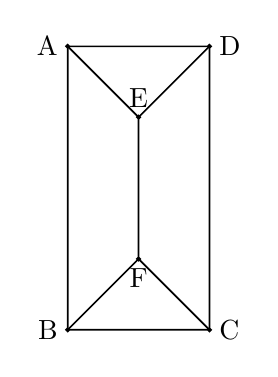
\begin{tikzpicture}[scale=0.3,line width=0.6pt]
	\draw
	(0,0) circle (2pt) node[left] {B} --
	(0,12) circle (2pt) node[left] {A} --
	(6,12) circle (2pt) node[right] {D} --
	(6,0) circle (2pt) node[right] {C} -- (0,0)
	(3,9) circle (2pt) node[align=left,   above] {E} --
	(3,3) circle (2pt) node[align=left, below] {F} ;
	\draw[-] (6,0)--(3,3)--(0,0)   (6,12)--(3,9)--(0,12);
	\end{tikzpicture}
\end{figure}

\end{frame}


%
%\begin{frame}
%\begin{quest}
%	证明$$\sum_{i=0}^{n}\binom{a}{i}\binom{b}{n-i}=\binom{a+b}{n},$$
%	其中$a, b, n$都是非负整数.
%\end{quest}
%\end{frame}




\begin{frame}
\begin{quest}
1与1000之间不能被5,6,8整除的整数有多少个?
\end{quest}

\begin{quest}
$n$对夫妇参加宴会围桌就座, 要求男女相间并且每对夫妇两人不得相邻, 问有多少种就座方式?
\end{quest}

\begin{quest}
由5个字母$a,b,c,d,e$构成的全排列中, $a$不能出现在$1,5$位置上, $b$不能出现在$2,3$位置上, $c$不能出现在$3,4$位置上, $e$不能出现在$5$位置上. 问有多少种排列方法?
\end{quest}
\end{frame}



\begin{frame}
\begin{quest}
证明任意$n^2+1$个实数组成的序列中, 必有一个长为$n+1$的递增子序列, 或必有一个长为$n+1$的递减子序列.
\end{quest}
\end{frame}

	\begin{frame}\frametitle{整数分拆}
正整数$n$的一个\alert{(无序)分拆}(Partitions)  $\lambda$是指一个单调不增的正整数序列$(\lambda_1,\lambda_2,\ldots,\lambda_k)$, 满足
$$
\lambda_1+\lambda_2+\cdots+\lambda_k=n.
$$

例如,
	$n=4$的所有分拆为
	$$
	(4),(3,1),(2,2),(2,1,1),(1,1,1,1).
	$$
\end{frame}


\begin{frame}\frametitle{杨表}
	杨表(Young tableau)是由杨(R.A.
	Young)在1901年研究不变量理论时引入的, 它在组合数学、群表示论、数学物理
	等领域中都有重要应用. 通常情况下, 杨表是指定义在
	杨图上的半标准杨表.

	给定一个整数分拆$\lambda=(\lambda_1,\lambda_2,
	\ldots,\lambda_k)$, 与$\lambda$对应的
	杨图(Young Diagram)定义为平面上一些左对齐的$k$行方块的集合,
	使得第$i$行恰有$\lambda_i$个方块. 例如, 分拆$(4,2,1)$对应的杨图为
	\begin{figure}[h]
		\setlength{\unitlength}{0.5mm}
		\begin{center}
			\begin{picture}(50,30)
			\put(0,30){\line(1,0){40}}\put(0,20){\line(1,0){40}}
			\put(0,20){\line(1,0){20}}\put(0,10){\line(1,0){20}}
			\put(0,0){\line(1,0){10}}\put(0,0){\line(0,1){30}}
			\put(10,0){\line(0,1){30}}\put(20,30){\line(0,-1){20}}
			\put(30,30){\line(0,-1){10}}\put(40,30){\line(0,-1){10}}
			\end{picture}
		\end{center}
	\end{figure}
\end{frame}



\begin{frame}\frametitle{标准杨表}
	设$\lambda$是$n$的一个分拆.
	在$\lambda$对应的杨图中, 用正整数填充图中的每个方块得到一个阵列$T$.
	若用${1,2,\ldots,n}$填充$\lambda$对应的杨图使得每个数字恰好出现一次,
	并且每行每列递增, 则称这样的阵列为具有形状$\lambda$的
	标准杨表SYT(standard Young tableau).
	例如下图是一个形状为$(4,2,1)$的标准杨表.
\begin{figure}[ht]
	\setlength{\unitlength}{0.5mm}
	\begin{center}
		\begin{picture}(50,30)
		\put(0,30){\line(1,0){40}}\put(0,20){\line(1,0){40}}
		\put(0,20){\line(1,0){20}}\put(0,10){\line(1,0){20}}
		\put(0,0){\line(1,0){10}}\put(0,0){\line(0,1){30}}
		\put(10,0){\line(0,1){30}}\put(20,30){\line(0,-1){20}}
		\put(30,30){\line(0,-1){10}}\put(40,30){\line(0,-1){10}}
		\put(4,22){1}  \put(14,22){3} \put(24,22){6}\put(34,22){7}
		\put(4,12){2}
		\put(14,12){5}
		\put(4,2){4}
		\end{picture}
	\end{center}
\end{figure}
\begin{quest}
	标准杨表(SYT)的个数
\end{quest}
\end{frame}



\begin{frame}
\begin{center}
\textbf{\Huge{\textcolor{blue}{Thanks for your attention!}}}
\end{center}
\end{frame}

\end{document}
